\subsubsection{Operación O1.1}

\begin{figure}[h!]
\centering
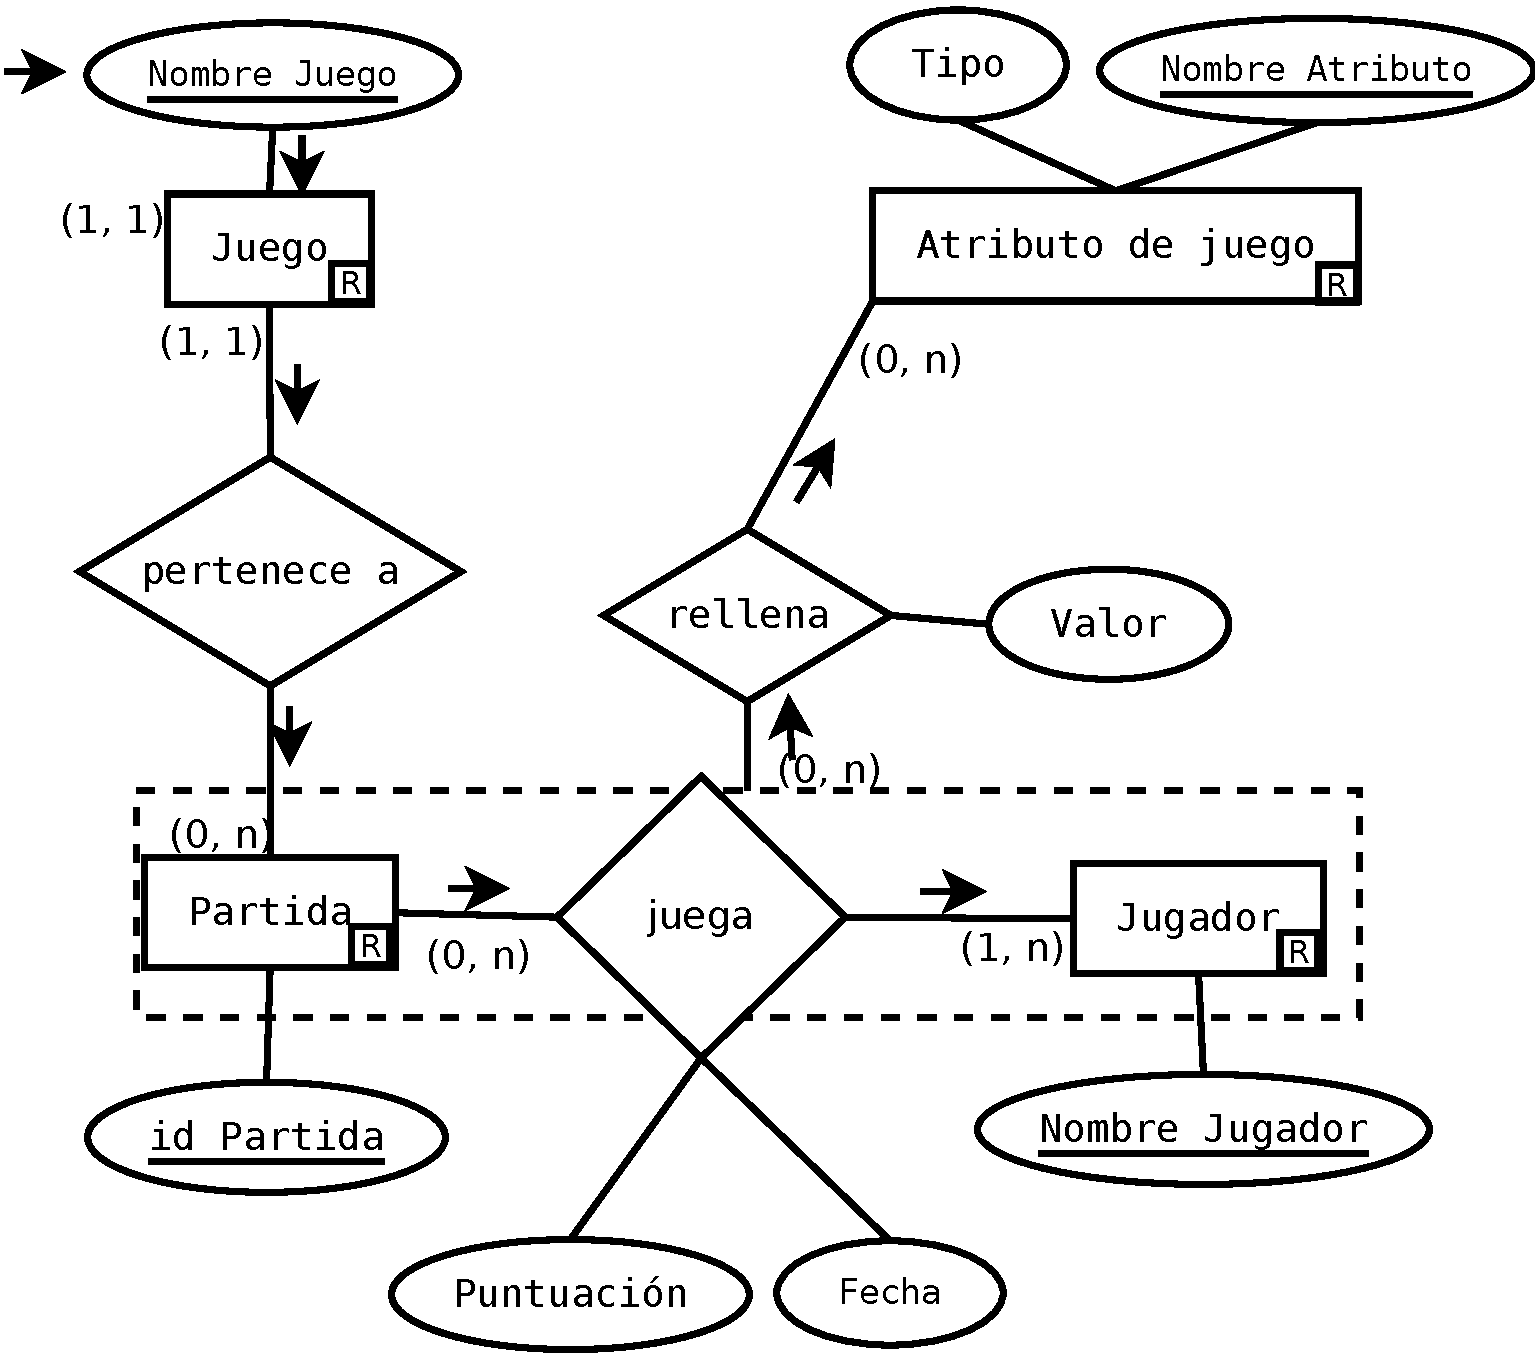
\includegraphics[width=0.7\linewidth]{../Diagramas/pdf/Op1-Consulta.pdf}
\caption{Esquema de navegabilidad de la operación O1.1.}

\label{fig:O1.1}
\end{figure}

\subsubsection{Operación O1.2, O1.3 y O1.4}

\begin{figure}[h!]
	\centering
	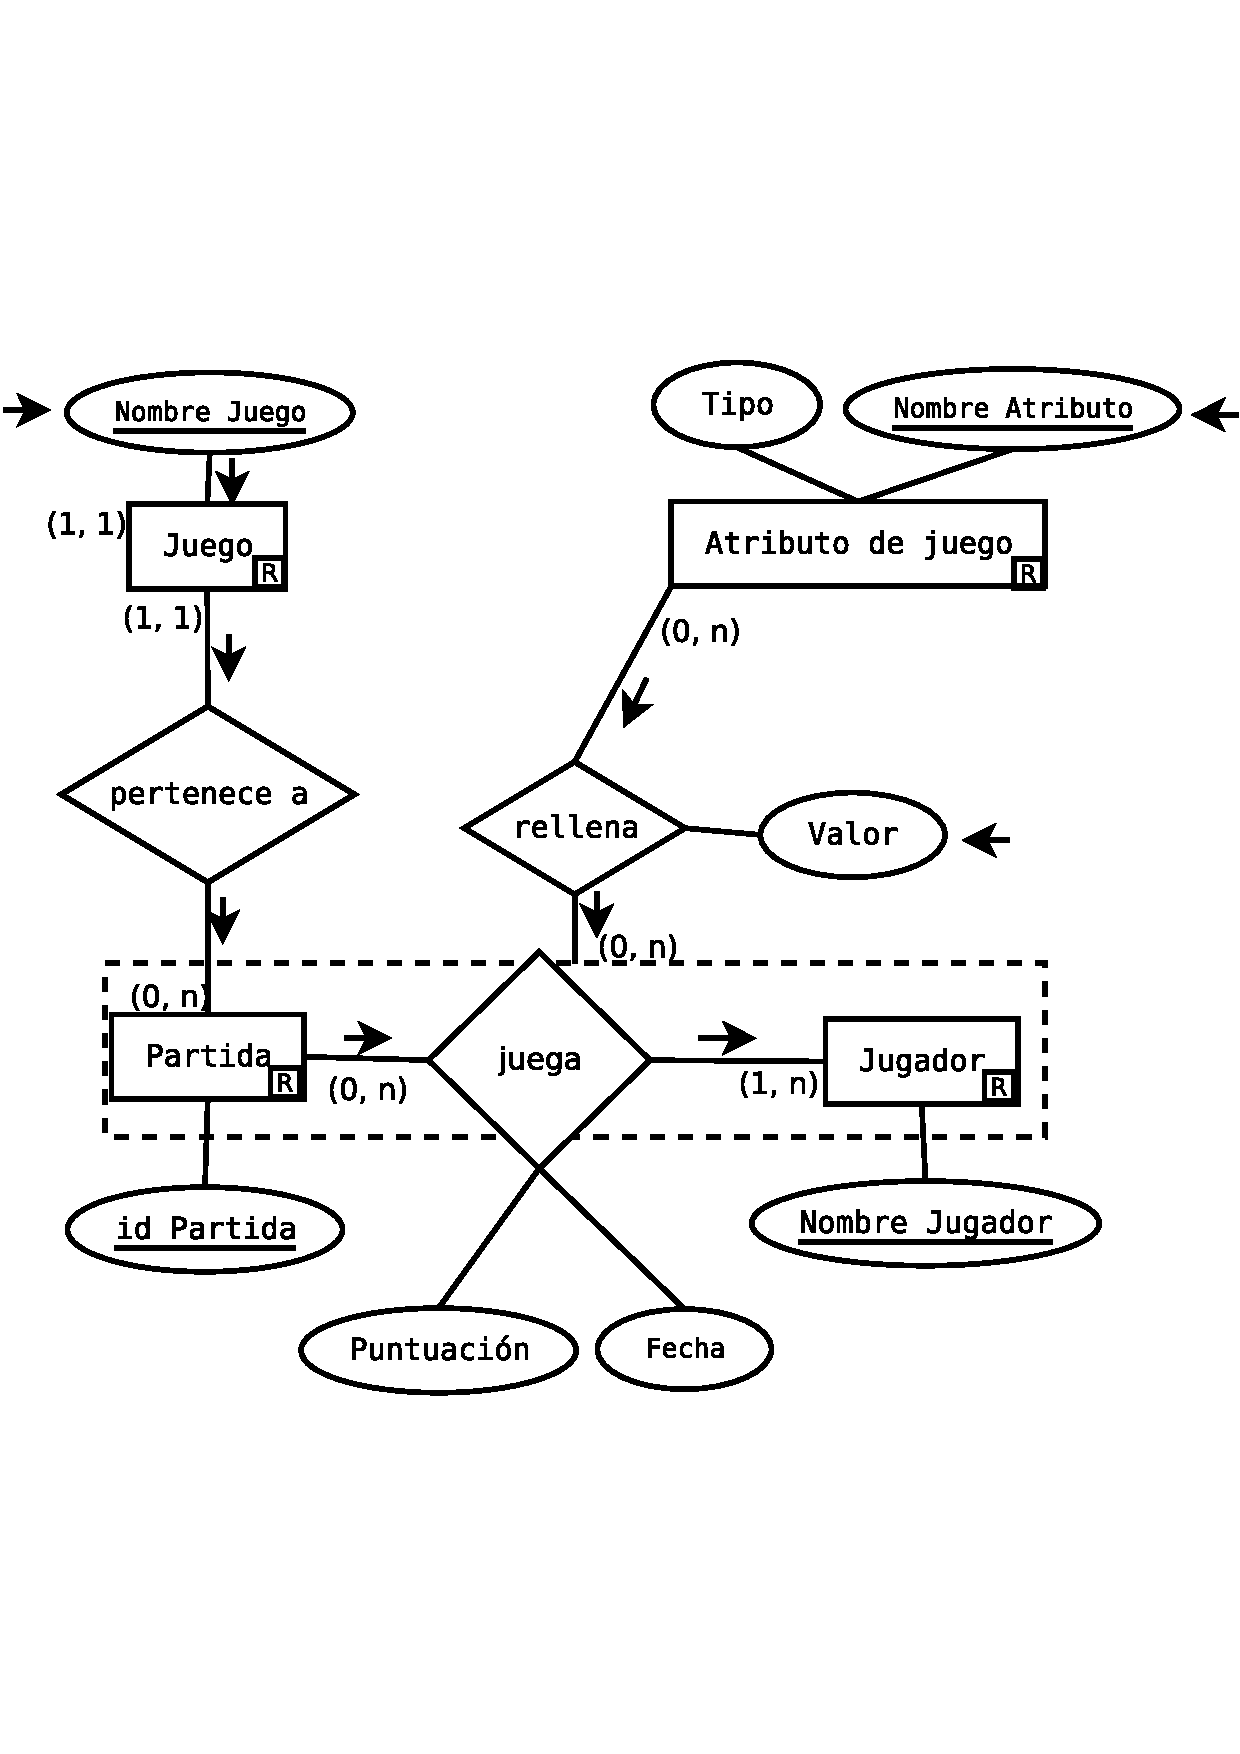
\includegraphics[width=0.7\linewidth]{../Diagramas/pdf/Op2-Consulta.pdf}
	\caption{Esquema de navegabilidad de la operación O1.2, O1.3 y O1.4.}
	
	\label{fig:O1.2}
\end{figure}

Especificaciones:
\begin{itemize}
	\item Cada atributo tiene un valor dependiendo de la propia partida, y para \textbf{O1.3} y \textbf{O1.4} se fijan varios atributos con un valor por cada atributo.
\end{itemize}
